\section{Early considerations}

We started with the initial assumption that the project can be divided into two challenges: Firstly, the classification, and secondly the localization. We found an approach that allows for both challenges to be addressed together relatively early on. Nonetheless we will firstly cover an early alternative approach, because it will help us showcase some inherent difficulties of the challenges that had to be overcome.

We firstly decided to approach this as a problem where the images are, in a certain way, of a too high resolution. We mean this in the sense that there are tools and tissue, with the tissue obscuring the tools. This of course is a rather naive assumption. We followed the approach of \cite{https://doi.org/10.48550/arxiv.1512.03385} to use a variational auto-encoder to reduce the images to little more than the tools, since those should be considered the most important parts of the image, or are at least the parts easiest to recognize for the De- and Encoder, since the tools appear more often than the respective tissue-structures. This type of unsupervised learning is appealing, but the output can be limited only to frequently occurring and visually consistent objects \citep{localization_free}, which might be the biggest underlying weakness of this approach.

\begin{figure}[H]
	\centering
	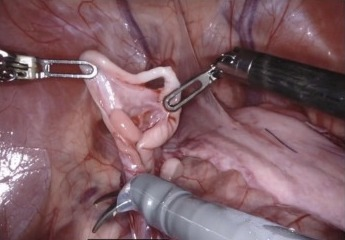
\includegraphics[width=10cm]{3_methodology/Tools}
	\caption{As one can imagine the tools do stand out - sometimes...}
	\label{fig:Tools_Good}
\end{figure}

\begin{figure}[H]
	\centering
	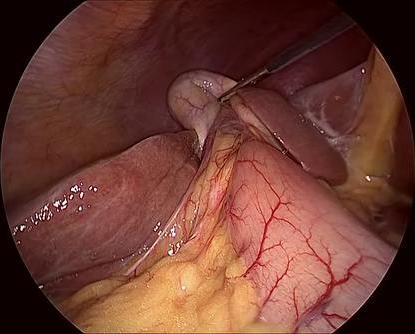
\includegraphics[width=10cm]{3_methodology/tools_bad}
	\caption{And sometimes not so much.}
	\label{fig:Tools_Bad}
\end{figure}

\cite{articleVAE} presented a relatively straightforward VAE-model, that we decided to rebuild and adapt to our needs \ref{fig:VAE}. 

\begin{figure}
	\centering
	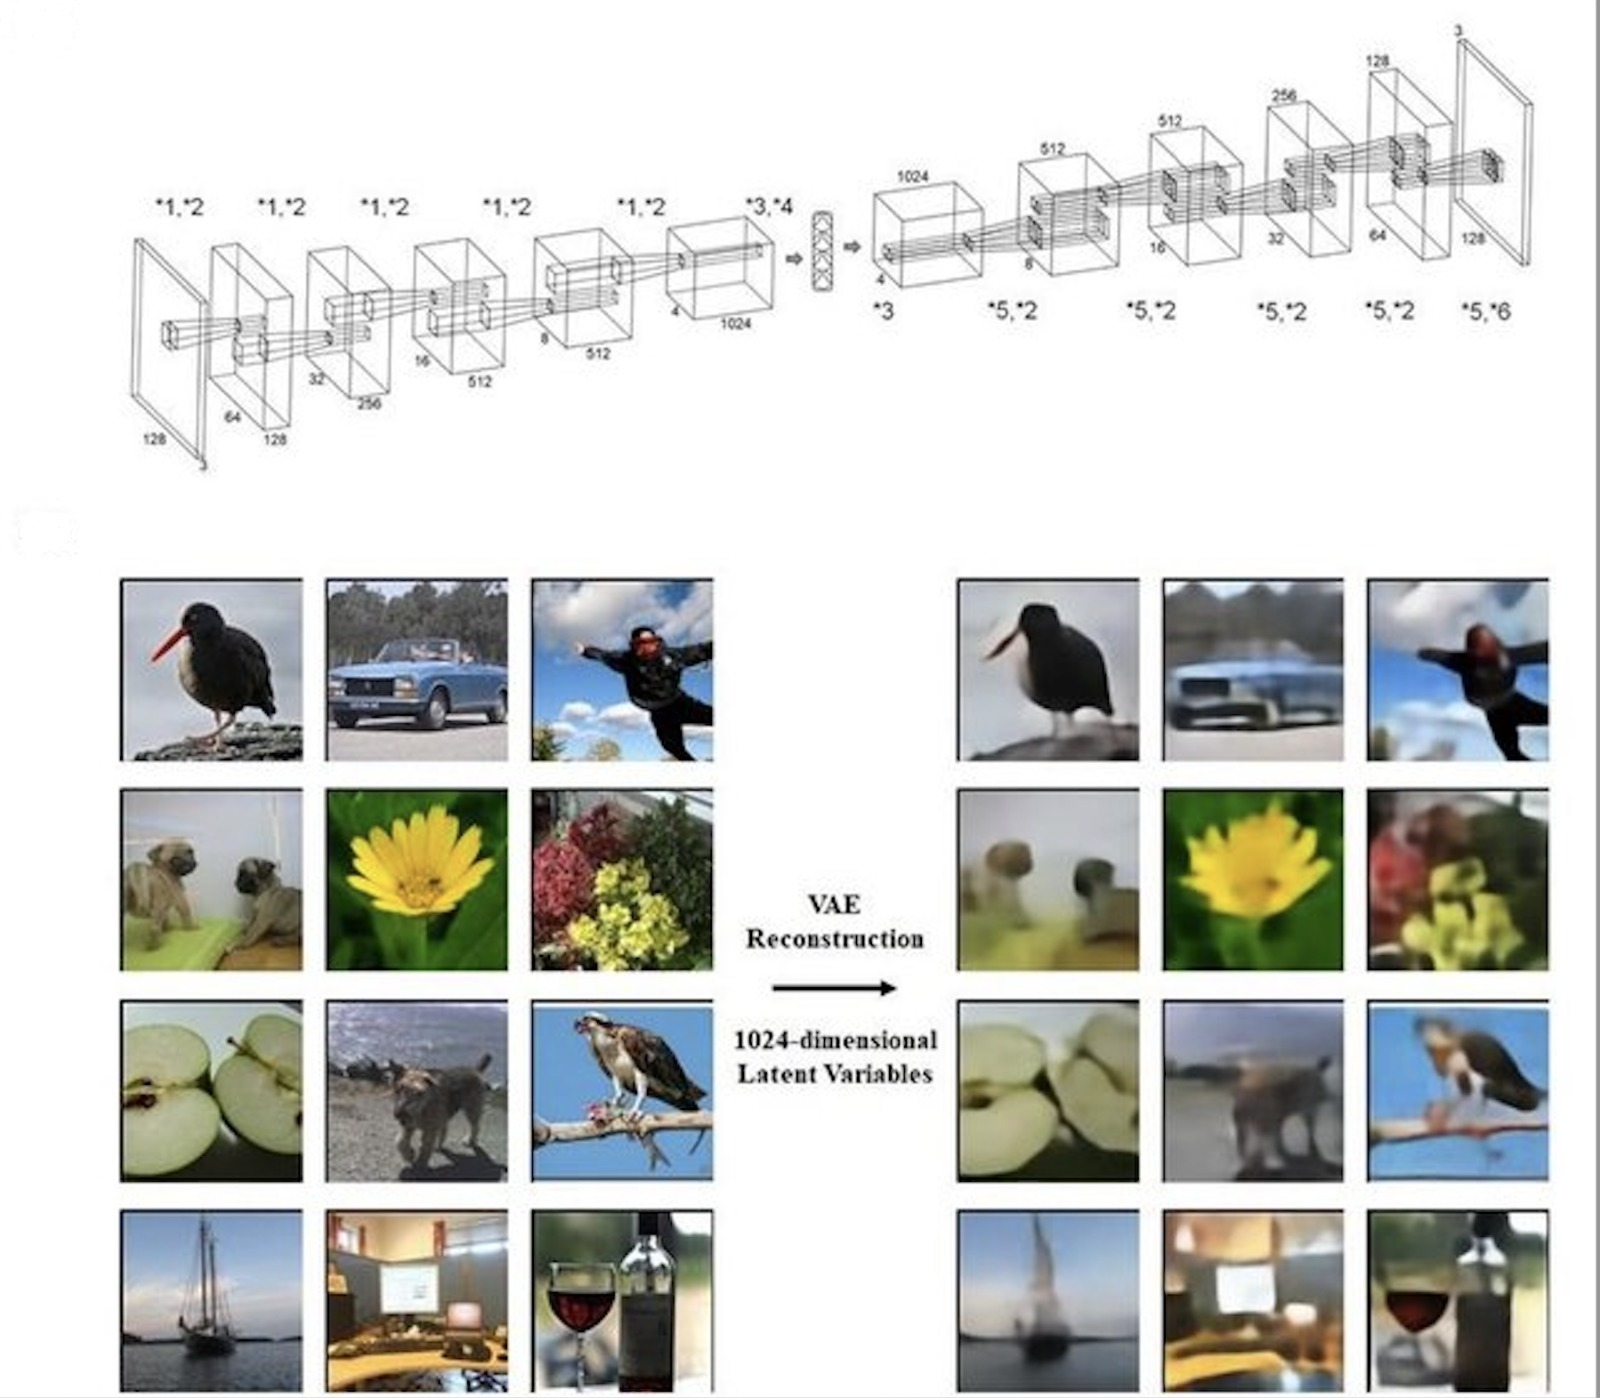
\includegraphics[width=10cm]{3_methodology/VAE_arch}
	\caption{Architecture (top) and result (bottom).}
	\label{fig:VAE}
\end{figure}


Since we don't need any representation that keeps too much of the original image, we mainly trimmed the whole approach down.
In the end, so we hoped. the instruments would be the parts that would at least to some extend be "saved over" to the other side of the image. We also experimented with the latent representation (or distribution, rather), hoping it might encode the information preserving locality, so that the interpretation of the representation gives clues already. For this purpose we settled at around 500 latent variables, since less would not be useful in terms of placing an object within an image. 

The more straightforward approach here is of course threading the image through a needle, meaning a rather small latent variable space again, and then analysing the reconstruction. The hope was that the image would preserve well distinguishable blobs where the tools were, so that we could filter the localization of the tools with some old-fashioned blob-detection via \href{https://en.wikipedia.org/wiki/Otsu%27s_method}{Otsus method} or similar approaches.

However, although the concept of VAEs is very intriguing, there is still an issue to address: Given a successful localization of objects, how does one classify the image?
The challenge is, that even when given only the part of the image with the tool itself, this would still leave us with having to solve a rather unpleasant classification problem, since all the images come annotated with all the classes originally in the image. This problem accompanied us during the whole project. The advantage in this case is, that we would stick with the well-known one-label-classification problem, meaning that ideally only one label is true at any point, although the calculation of the loss would be difficult. We are confident that this problem would have been solvable as well. But searching for a solution for the image-classification-part, we found that there was already a better approach.

\section{Data management}

We build a first prototype of the VAE, but training was impossible at first due to the handling of the huge dataset that we used first, that comprised of over 100GB of image data. More on that in the experimentation section. However, the sheer amount of data was not the main issue, but it points to a different one: We could not simply take the data, split it up into a training-, validation- and test-set and perform SGD on the training-set. 
This has two reasons: Firstly, the data was very unbalanced (see \ref{fig:surgtoolloc_tool_frequencies}). Secondly, and more importantly, we had to somehow make sure that the model would not learn something else, an issue that can be illustrated by some funny and some rather \href{https://www.forbes.com/sites/korihale/2021/09/02/ai-bias-caused-80-of-black-mortgage-applicants-to-be-denied/}{sinister examples}.

To this end we flipped the image with a 50\% chance, rotated it between -90 and 90 degrees, masked and cropped the images. Masking means that we set some regions of the image to the mean value of the rest of the dataset \citep{hideandseek}. The regions were selected in the following way: Any image was divided into 24x24-tiles, with every tile having a 50\% chance of being masked. Since this is basically the binomial distribution we can expect that around half of the tiles are masked everytime. This can look like this:

\begin{figure}[H]
	\centering
	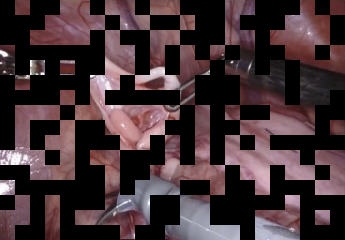
\includegraphics[width=10cm]{3_methodology/masked}
	\caption{Example for a masked image.}
	\label{fig:Masked}
\end{figure}


Another measure covered in the lecture on data-augmentation was the fact, that some falsely-annotated data put into the training-set might also serve the generalization-abilities of the network. We decided against any such measure, since the multi-classification of the entire clip presented us with more falsely annotated images than we might have wished for.

Having the data handled we went on exploring possible solutions to classifying the images. We therefore turned to CNNs, that, as we covered in the lecture, proved quite useful in image-classification-challenges. One interesting aspect of CNNs like the ResNET-models is that, before reducing the output of the last hidden layer to logits of the class-probabilities, these models preserve some of the size and locality of the input since the transformations are mainly convolutional in character. This means that the ResNets forward-pass can be intercepted, while the locality of the discovered features is preserved.
This also means that by computing a fully connected convolution one gets a heatmap for all the tools \citep{classpeak}. This procedure is fairly common already (see section 2.2). It is quite obvious that a well-performing network that returns heatmaps of the tools presence renders any other effort to localize tools obsolete. Since this is the concept we eventually pursued, we will cover it in more detail:

\section{The final model}
For the underlying architecture of the final model we followed a straightforward and established approach: We worked with a well-performing backbone to extract features of the image and trained a convolutional layer with kernel size 1x1 based off of those features. This results in a heatmap, that can be further processed.
The fully connected convolutional layer thereby replaces the sliding-window-approach, because it essentially performs the work of a fully-connected layer on a small part of the image, but, exploiting the convolutional nature of the layer, more efficiently than iterating with a fully connected layer over parts of the image over and over again. 

Using backbones is so successful because although those we used were originally applied to other image-classification-tasks, it appears that until the last few layers, the main work that is being done by the net is extracting features within the image. This leaves the task of "making sense" of these features to the last layer \citep{Vardazaryan}. The opportunity therefore lies in the possibility of omitting these last layers, and to train only the last layer for the specific task at hand (see for example the paper by \cite{https://doi.org/10.48550/arxiv.2206.08016}). As they point out, there are certain networks that have become common choices.
We tried and experimented with three backbones, each of which come with different depths: The ResNet by \cite{https://doi.org/10.48550/arxiv.1512.03385}, the AlexNet by \cite{krizhevsky2017imagenet} and the VGG net by \cite{https://doi.org/10.48550/arxiv.1409.1556}.
All three of them are readily available via the PyTorch-libraries.

We will cover the advantages of the different backbones more thoroughly in the experiment section, since the use of different nets can be understood as a hyper-parameter to optimize.

The localization and classification of the tools is being determined via the heatmaps: The network returns one heatmap for each class. Firstly, it is being decided via a pooling-layer which classes are present. The pooling functions are considered a hyper-parameter, although the use of an min-max-pooling in the ResNet-architecture left us with a good starting point. After having decided which heatmaps to consider, we eventually chose the peaks in these maps as the place of the object. This differs from the SurgTool-challenge, where they want bounding boxes, but proved easier to compare to existing literature like the extremely helpful paper by \cite{Vardazaryan} (section 3.4).

Taken altogether we ended up using a ResNet-18-backbone with stride 2$\times$2 with a 1$\times$1-kernel convolution-layer to generate the heatmaps for the classes and min-max-pooling for classification.

\section{Training}

The training was carried out using mini-batch stochastic gradient descent with different batch sizes, ranging from 2 to 50. We monitored both training and validation losses as well as average precision and accuracy.  After every iteration over the dataset we validated the training progress on a completely separate set.
As mentioned earlier, contrary to what we were used to we looked at a multi-label-classification problem. This had to be taken into account when choosing a loss function. We went with the multi-label soft margin loss, a weighted cross-entropy loss presented in equation \ref{Equ1}, where $k_c$ and $v_c$ are the ground truth and predicted tool presence for class $c$, $\sigma$ is the sigmoid-function and $W_c$ is the weight for class $c$. The weights serve as a counter-measure against the effect of class-imbalances (discussed in section 4.1).

\begin{align}
	Loss = \sum_{c=1}^C\frac{-1}{N}[W_ck_clog(\sigma(v_c)) + (1+k_c)log(1-\sigma(v_c))]\label{Equ1}
\end{align}


\subsection{Training workflow}

Training a neural network is challenging and resource-draining. Therefore developing a code base and workflow to overcome these problems is not a trivial task and should be considered part of the overall effort. 

We used ColabPro to compute the training. Doing so means that both the data and the code-files must be uploaded into a Google-Drive-account and then be run using
\newline \textbf{\%run train.py -...} 
\newline This implies one main requirement, namely that the hyper-parameters should be easy to change without touching the code base. We did this using configuration-files. They have been implemented to choose different compositions of backbones, convolutional layers and hyper-parameters like the strides of the convolutional layer. We also implemented means of saving the trained parameters and resuming the process at any time, even keeping a history of the different states, as well as utility-functions that kept us up-to-date about the training progress. More on these in the quality metrics-section. 

\subsection{Hyper-parameter tuning}
We tuned the following hyper parameters: 
We did so by training 16 combinations for each 50 epochs on a smaller dataset, during each epoch we collected the quality metrics of each for each parameter-combination and epoch. Based off of these data points we ran a gaussian process by iterating over a much tighter net of hyper parameters, searching for a combination that appeared promising in terms of further training. We picked the gaussian process from the sklearn-library and went with the recommended parameters.
The main difficulty that emerged using this process is that we had to assign a value to the data points that we collected for each combination of parameters. It seems important to take not just the best-performing model at any epoch, but also a model that shows continued improvement as well as overall good performance. We tried different approaches, but stuck to a simple one by calculating the mean and adding the weighed minimum to it. 

Apart from that we just had to try some options intuitively, especially which pooling-function or backbone to use. This will be one main part of the experiment section.

\section{Quality metrics}

We used the precision-recall-curve, the F1-score (that merely combines the precision- and recall-values), the average precision, the average distance between a bounding box centre and the closest correct predictions in percent of the diagonal length (for localization). The average precision metric was also used to interpret the localization performance. All these metrics were applicable, since we took care in balancing the classes, which is, at least for the classification part, an important prerequisite. Some of the metrics provide redundant information (especially true for the F1-score and the precision-recall-metric), although some of them are easier to interpret on the spot. But it does not seem to hurt to in doubt calculate more metrics than necessary.
When it comes to assess the quality of the model, we mainly looked towards papers that covered similar problems. For instance, \cite{Vardazaryan} used average precision to evaluate the binary tool presence classification as well as the localization. We not only looked at these papers for inspiration, but also as a benchmark we wanted to achieve as well, meaning that average precision of over 90\% for all tools was the overall goal (as achieved by \cite{Vardazaryan}, \cite{endonet} and \cite{lstm}).

